{\color{gray}\hrule}
\begin{center}
\section{Results} \label{sec:results}
\bigskip
\end{center}
{\color{gray}\hrule}

\begin{multicols}{2} 
The mass of the weights were calculated using digital weights: $M = 29.9 \pm 0.1 (g)$.
\begin{equation} \label{eq:results:weight}
  \left\langle M \right\rangle = \frac{1}{N}\sum\limits_{i=1}^{N}M_{i} = 29.9 (g)
\end{equation}
\begin{equation} \label{eq:results:weight_err}
  \Delta M = \frac{1}{N}\sqrt{\sum\limits_{i=1}^{N}(M_{i} - \left\langle M \right\rangle)^{2}} = 0.1 (g)
\end{equation}

As discussed in section \ref{sec:methods}, weights were attached to either ends of the gyroscope. However, weight's position was pushed towards the gyroscope vertical axis due to rotations (see figure \ref{fig:results:locs}). Three possible locations were measured using vernier callipers to be:
\begin{equation*}
  \left\langle l_{I} \right\rangle = \frac{1}{N}\sum\limits_{i=1}^{N}l_{Ii} = 33.0 (cm)
\end{equation*}
\begin{equation} \label{eq:results:l_err}
  \Delta l_{I} = \frac{1}{N}\sqrt{\sum\limits_{i=1}^{N}(l_{Ii} - \left\langle l_{I} \right\rangle)^{2}} = 0.4 (cm)
\end{equation}

Thus, $l_{I} = 33.0 \pm 0.4 (cm)$. Similarly, $l_{II} = 19.7 \pm 0.1 (cm)$ and $l_{III} = 23.9 \pm 0.1 (cm)$.

\emph{TISensorTag} was recording precession frequency ($\boldsymbol\Omega$) of the gyroscope (vertical axis) for different torques\footnote{Torque is specified by the mass of the weight and the lever arm length where the weight was attached with respect to the vertical axis of the gyroscope.} and different spinning angular velocities $\boldsymbol\omega_{3}$. This data is shown in table \ref{tab:results:precession} for each point (see appendix \ref{sec:appendix:precession_raw_data} for more details about precession frequency data, and appendix \ref{appendix:errors} for detailed error analysis).

\end{multicols}

\begin{table}[H]
  \centering
  \begin{tabular}{|c|c|c|c|c|}
    Point & Type & Precession ($\boldsymbol\Omega$), $\frac{rad}{s}$ & Mass ($M$), $g$ & Lever Arm Length ($l$), $cm$ \\ \hline
    $\#1$ & $II$ & $0.449711 \pm 0.031443$ & $59.8 \pm 0.2$ & $19.7 \pm 0.1$ \\ \hline
    $\#2$ & $II$ & $0.716604 \pm 0.055174$ & $59.8 \pm 0.2$ & $33.0 \pm 0.4$ \\ \hline
    $\#3$ & $II$ & $0.18821 \pm 0.02623$   & $29.9 \pm 0.1$ & $23.9 \pm 0.1$ \\ \hline
    $\#4$ & $II$ & $0.56268 \pm 0.06639$   & $59.8 \pm 0.2$ & $33.0 \pm 0.4$ \\ \hline
    $\#5$ & $I$  & $0.528033 \pm 0.005273$ & $29.9 \pm 0.1$ & $33.2 \pm 0.4$ \\ \hline
    $\#6$ & $I$  & $0.258233 \pm 0.002976$ & $29.9 \pm 0.1$ & $33.2 \pm 0.4$ \\ \hline
    $\#7$ & $I$  & $0.165118 \pm 0.000843$ & $59.8 \pm 0.2$ & $19.7 \pm 0.1$ \\ \hline
  \end{tabular}
  \caption{Precession frequencies ($\Omega$)}
  \label{tab:results:precession}
\end{table}

\begin{multicols}{2}
 In the first part of the experiment the rotor’s behavior without external forces was observed, for this the rotor was rotated by hand. After this the base was rotated, during the rotation of the base the rotor remained stationary. This is caused by conservation of angular momentum (see section \ref{sec:discussion:no} for further details).
  
\begin{figure}[H]
  \centering
  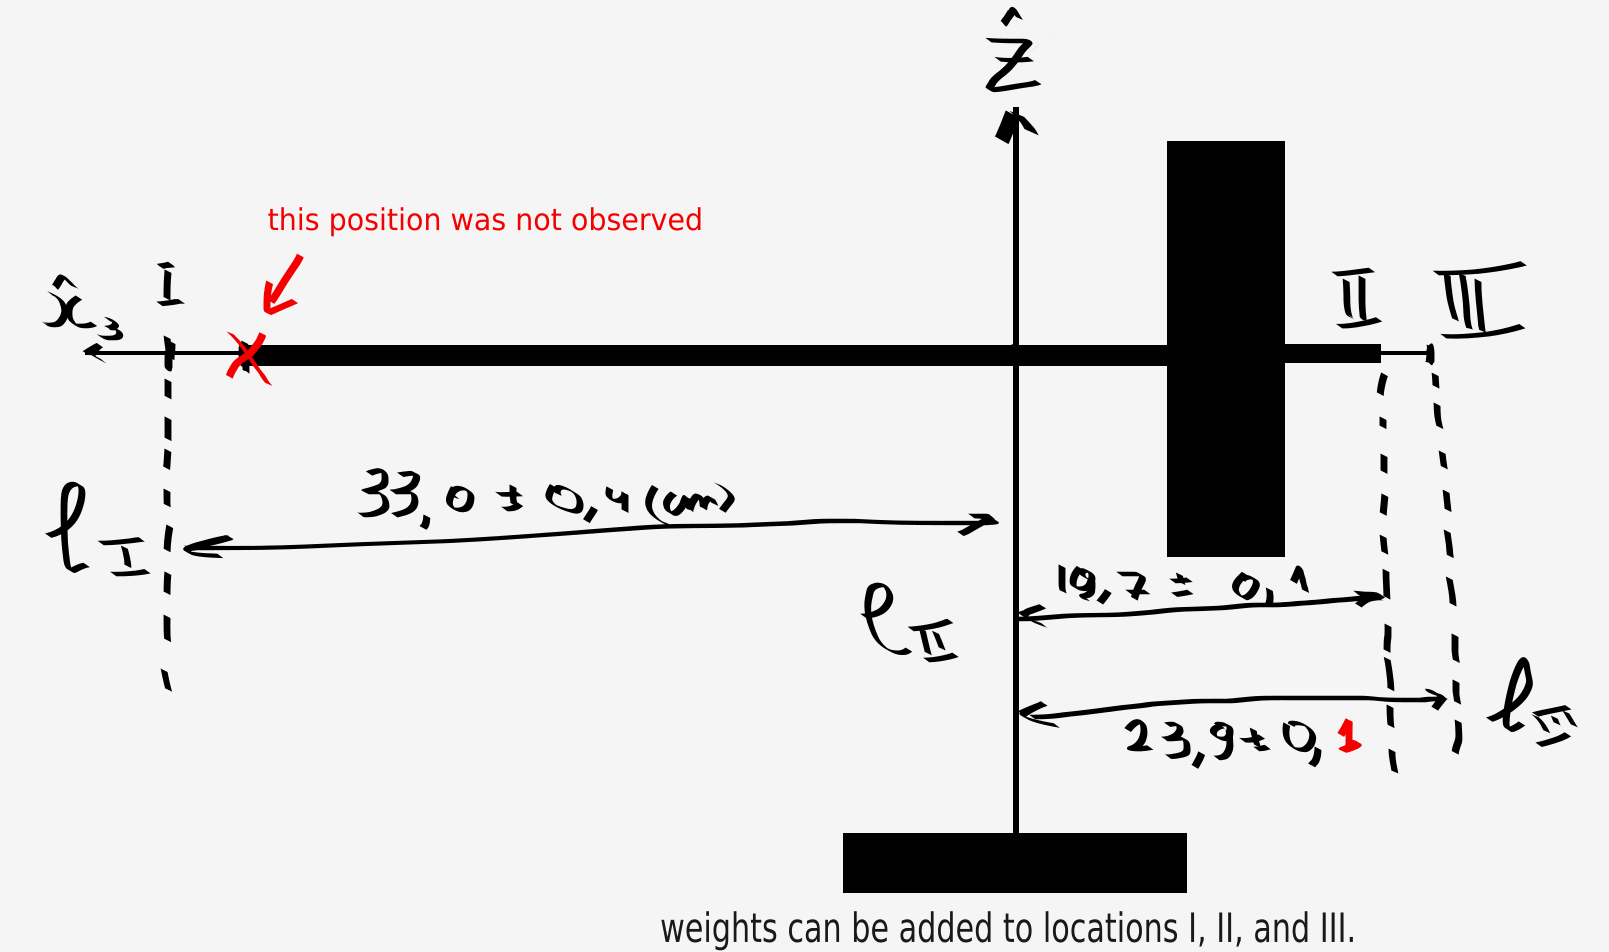
\includegraphics[width=\columnwidth]{gyroscope/images/locs}
  \caption{Possible weights locations on the gyroscope's rotor axis. }
  \label{fig:results:locs}
\end{figure}

The gyroscope would only precess if torque was applied to it, this was done by adding weights to the setup. The weight had a mass of $29.9 \pm 0.1 (g)$ (see equation \ref{eq:results:weight} and \ref{eq:results:weight_err}), the masses were placed at distances of $l_{I}$, $l_{II}$ and $l_{III}$ from the vertical axis of the gyroscope.
Next, rotor's moment of inertia around its own axis ($\hat{x}_{3}$) was determined, this was done using equation \ref{eq:theory:id},
where $M_d = 1.74 (kg)$ is the mass of the rotor disc and $R_d = 12.47 \pm 0.04 (cm)$ is the radius of the disc. Substituting in the values of $M_d$ and $R_d$ gave $I_3 = 0.0271 \pm 0.0004 (kg \cdot m^2)$. After this, $T_3$ was calculated by the following equation:
\begin{equation*}
    T_3 = \frac{10}{A_{r}}
\end{equation*}
where $A_{r}$ is the average number of rotations per 10 seconds, which was determined by filming the setup and dividing the film in $10$ second long clips, counting the rotations per clip and then taking the average. The previous measured components were used to calculate $T_{p, \text{calculated}}$ using equation \ref{eq:theory:precession_period}. $T_{p, \text{measured}}$ was calculated using:
\begin{equation*}
    T_{p, \text{measured}} = \frac{2\pi}{\Omega}
\end{equation*}
$T_{p, \text{calculated}}$ was plotted against $T_{p, \text{measured}}$ in figure \ref{fig:gyro}.

\begin{figure}[H]
    \centering
    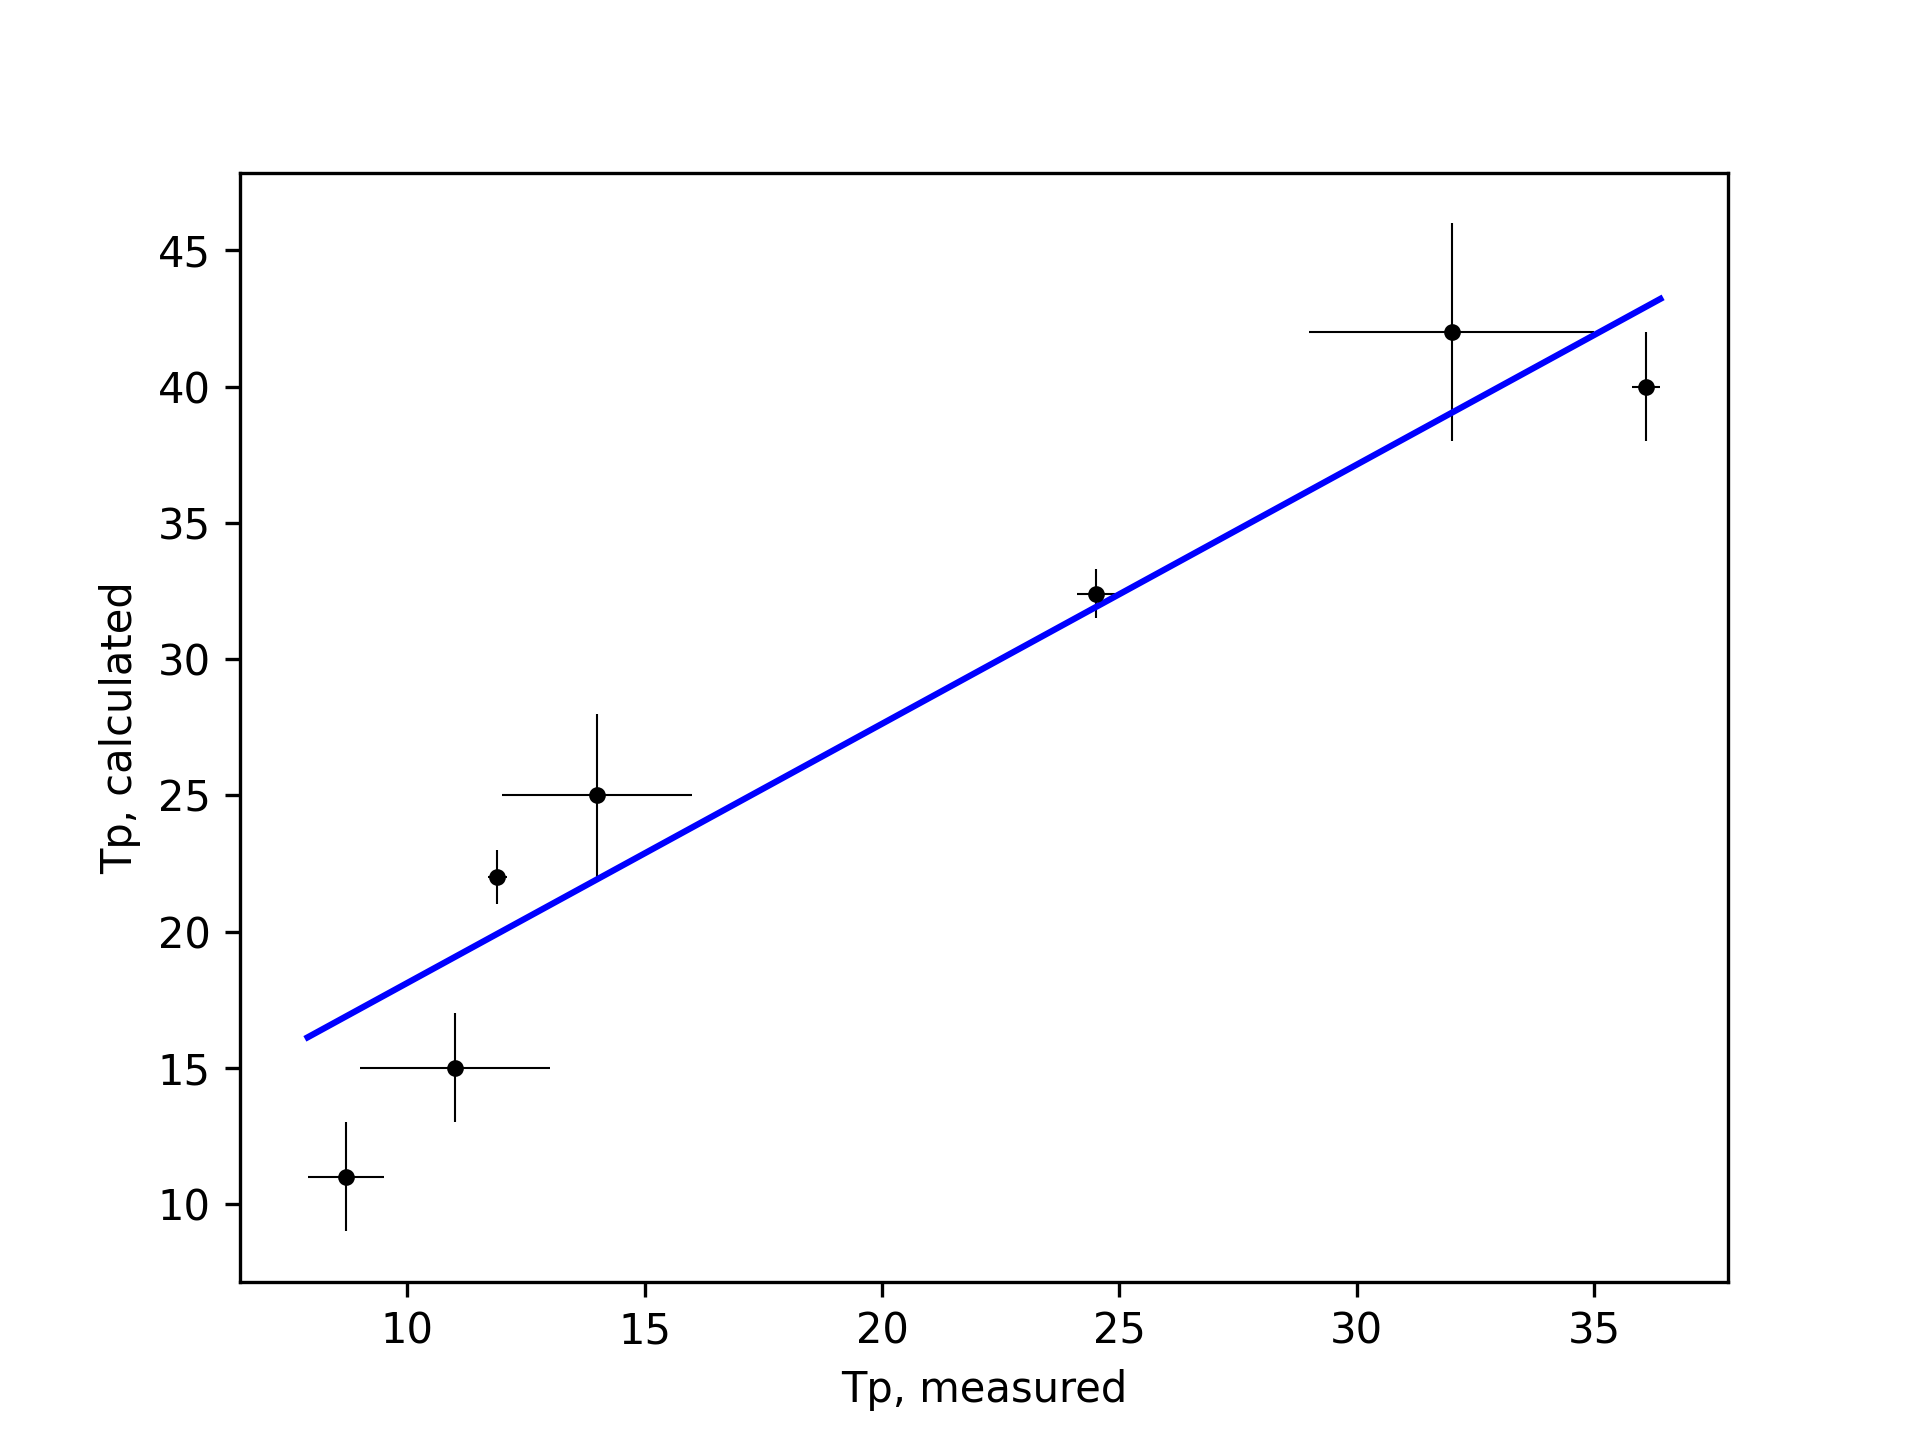
\includegraphics[width=\columnwidth]{gyroscope/images/gyro}
    \caption{Correlation between calculated and measured precession periods}
    \label{fig:gyro}
\end{figure}

The line of best fit has a slope of
\begin{equation}
  \label{eq:results:slope}
  \Delta \theta = 1.0 \pm 0.2 (rad)
\end{equation}

\end{multicols}
